%%%%%%%%%%%%%%%%%%%%%%%%%%%%%%%%%%%%%%%%%%%
%
% From a template maintained at https://github.com/jamesrobertlloyd/cbl-tikz-poster
%
%%%%%%%%%%%%%%%%%%%%%%%%%%%%%%%%%%%%%%%%%%%

\documentclass[portrait,a0b,final,a4resizeable]{a0poster}
\setlength{\paperwidth}{36in} % A0 width: 46.8in
\setlength{\paperheight}{48in} % A0 width: 46.8in

\usepackage{atbegshi}% http://ctan.org/pkg/atbegshi
\AtBeginDocument{\AtBeginShipoutNext{\AtBeginShipoutDiscard}}
\usepackage{qrcode}
\usepackage{multicol}
\usepackage{enumitem}
\usepackage{mathtools}
%\usepackage{color}
%\usepackage{morefloats}
%\usepackage[pdftex]{graphicx}
%\usepackage{rotating}
\usepackage{amsmath, amsthm, amssymb, bm}
%\usepackage{array}
%\usepackage{booktabs}
\usepackage{multirow}
%\usepackage{hyperref}
\usepackage{pgf-soroban}
\usepackage{bussproofs}
\usetikzlibrary{cd,shapes.geometric,arrows,chains,matrix,positioning,scopes,calc}
\tikzstyle{mybox} = [draw=white, rectangle]
%\definecolor{darkblue}{rgb}{0,0.08,0.45}
%\definecolor{blue}{rgb}{0,0,1}
%\usepackage{dsfont}
\usepackage[margin=0.5in]{geometry}
%\usepackage{fp}

%%%%%%%%%%%%%%%%%%%%%%%%%%%%%%%%%%%%%%%%%%%
%
% myfig
%
% \myfig - replacement for \figure
% necessary, since in multicol-environment
% \figure won't work
%
%%%%%%%%%%%%%%%%%%%%%%%%%%%%%%%%%%%%%%%%%%%

\newcommand{\myfig}[3][0]{
\begin{center}
    \vspace{1.5cm}
    \includegraphics[width=#3\hsize,angle=#1]{#2}
    \nobreak\medskip
\end{center}}

%%%%%%%%%%%%%%%%%%%%%%%%%%%%%%%%%%%%%%%%%%%
%
% mycaption
%
% \mycaption - replacement for \caption
% necessary, since in multicol-environment \figure and
% therefore \caption won't work
%
%%%%%%%%%%%%%%%%%%%%%%%%%%%%%%%%%%%%%%%%%%%

%\newcounter{figure}
\setcounter{figure}{1}
\newcommand{\mycaption}[1]{
\vspace{0.5cm}
\begin{quote}
{{\sc Figure} \arabic{figure}: #1}
\end{quote}
\vspace{1cm}
\stepcounter{figure}
}

%%%%%%%%%%%%%%%%%%%%%%%%%%%%%%%%%%%%%%%%%%%
%
% Some standard colours
%
%%%%%%%%%%%%%%%%%%%%%%%%%%%%%%%%%%%%%%%%%%%

\definecolor{camlightblue}{rgb}{0.601 , 0.8, 1}
\definecolor{camdarkblue}{rgb}{0, 0.203, 0.402}
\definecolor{camred}{rgb}{1, 0.203, 0}
\definecolor{camyellow}{rgb}{1, 0.8, 0}
\definecolor{lightblue}{rgb}{0, 0, 0.80}
\definecolor{white}{rgb}{1, 1, 1}
\definecolor{whiteblue}{rgb}{0.80, 0.80, 1}

%%%%%%%%%%%%%%%%%%%%%%%%%%%%%%%%%%%%%%%%%%%
%
% Some look and feel definitions
%
%%%%%%%%%%%%%%%%%%%%%%%%%%%%%%%%%%%%%%%%%%%

\setlength{\columnsep}{0.03\textwidth}
\setlength{\columnseprule}{0.0018\textwidth}
\setlength{\parindent}{0.0cm}

%%%%%%%%%%%%%%%%%%%%%%%%%%%%%%%%%%%%%%%%%%%
%
% \mysection - replacement for \section*
%
% Puts a pretty box around some text
% TODO - any other thoughts for what this box should look like
%
%%%%%%%%%%%%%%%%%%%%%%%%%%%%%%%%%%%%%%%%%%%

\tikzstyle{mysection} = [rectangle,
draw=none,
shade,
outer color=camlightblue!30,
inner color=camlightblue!30,
text width=0.965\columnwidth,
text centered,
rounded corners=20pt,
minimum height=0.09\columnwidth]

\newcommand{\mysection}[1]
{
\begin{center}
    \begin{tikzpicture}
        \node[mysection] {\sffamily\bfseries\LARGE#1};
    \end{tikzpicture}
\end{center}
}

%%%%%%%%%%%%%%%%%%%%%%%%%%%%%%%%%%%%%%%%%%%
%
% Set the font
%
% TODO - Not sure what a canonical choice is - feel free to modify
%
%%%%%%%%%%%%%%%%%%%%%%%%%%%%%%%%%%%%%%%%%%%

\renewcommand{\familydefault}{cmss}
\sffamily

%%%%%%%%%%%%%%%%%%%%%%%%%%%%%%%%%%%%%%%%%%%%%%%%%%%%
%%%               Background                     %%%
%%%%%%%%%%%%%%%%%%%%%%%%%%%%%%%%%%%%%%%%%%%%%%%%%%%%

\newcommand{\background}[3]{
%\definecolor{cgradbegin}{#1}
%\definecolor{cgradend}{#2}
% \psframe[fillstyle=gradient,gradend=cgradend,
% gradbegin=cgradbegin,gradmidpoint=#3](0.,0.)(1.\textwidth,-1.\textheight)
}




%%%%%%%%%%%%%%%%%%%%%%%%%%%%%%%%%%%%%%%%%%%%%%%%%%%%
%%%                pcolumn                       %%%
%%%%%%%%%%%%%%%%%%%%%%%%%%%%%%%%%%%%%%%%%%%%%%%%%%%%

\newenvironment{pcolumn}[1]{
\begin{minipage}{#1\textwidth}
\begin{center}
}{
\end{center}
\end{minipage}
}



%%%%%%%%%%%%%%%%%%%%%%%%%%%%%%%%%%%%%%%%%%%%%%%%%%%%
%%%                pbox                          %%%
%%%%%%%%%%%%%%%%%%%%%%%%%%%%%%%%%%%%%%%%%%%%%%%%%%%%

\definecolor{lcolor}{rgb}{0, 0, 0.80}
\definecolor{gcolor1}{rgb}{1, 1, 1}
\definecolor{gcolor2}{rgb}{.80, .80, 1}

% \def\fc{fillcolor}
% \def\getfc #1=#2\par{\def\ffc{#1} \ifx\ffc\fc #2\fi}
% \def\getfillcolor #1,#2\par{\getfc #1\par \getfc #2\par}

%  \newcommand{\psshadowbox}[2]{%[2][magenta]{
%      \fbox{Input arg: #1}
%      \fbox{#1}
%      \fbox {\getfillcolor #1\par}
%      \def\col{\getfillcolor #1\par}

%      \let\coll=\col
%       \coll
%     \colorbox{\col}{#2}
%       \mbox
%   \coloredshadowbox{black}{\coll}{#2}
%   }

\newcommand{\pbox}[4]{
%\psshadowbox[#3]{
%\fbox{
\mbox{
\begin{minipage}[t][#2][t]{#1}
#4
\end{minipage}
}%}
}

%%%%%%%%%%%%%%%%%%%%%%%%%%%%%%%%%%%%%%%%%%%
%
% Poster environment
%
% Centres everything and can be used to define the width of the content
%
%%%%%%%%%%%%%%%%%%%%%%%%%%%%%%%%%%%%%%%%%%%

\newenvironment{poster}{
\begin{center}
\begin{minipage}[c]{\textwidth}
}{
\end{minipage}
\end{center}
}

\def\newarrow{\mbox{\begin{tikzpicture}
\useasboundingbox{(-3pt,-4.5pt) rectangle (19pt,1pt)};
\draw[->] (0,-0.07)--(17pt,-0.07);\end{tikzpicture}}}

%%%%%%%%%%%%%%%%%%%%%%%%%%%%%%%%%%%%%%%%%%%
%
% Bottom box
%
%%%%%%%%%%%%%%%%%%%%%%%%%%%%%%%%%%%%%%%%%%%

\newlength{\bottomboxheight}
\setlength{\bottomboxheight}{0.1\paperheight}

\newcommand{\bottombox}[1]{\vfill
\noindent\colorbox{white}{
\begin{minipage}[c][\bottomboxheight][c]{\textwidth}
\centering
\begin{minipage}{0.9\textwidth}
\vfill{

\fontsizesection\color{black}
#1
}

\end{minipage}
\end{minipage}

}
}

%% Bottom box logo
\newcommand{\bottomboxlogo}[2][width=\textwidth]{
\begin{minipage}[c][\bottomboxheight][c]{0.3\textwidth}
\raggedleft\includegraphics[#1]{#2}
\end{minipage}
}

\newcommand{\bottomboxlogoleft}[2][width=\textwidth]{
\begin{minipage}[l][\bottomboxheight][c]{0.3\textwidth}
\raggedleft\includegraphics[#1]{#2}
\end{minipage}
}

%%%%%%%%%%%%%%%%%%%%%%%%%%%%%%%%%%%%%%%%%%%
%
% Highlighting
%
%%%%%%%%%%%%%%%%%%%%%%%%%%%%%%%%%%%%%%%%%%%

\definecolor{slightgray}{rgb}{0.90, 0.90, 0.90}

\usepackage{soul}
\makeatletter
\def\SOUL@hlpreamble{%
\setul{}{3.0ex}%
\let\SOUL@stcolor\SOUL@hlcolor%
\SOUL@stpreamble%
}
\makeatother

\newcommand{\inline}[1]{%
\begingroup%
\sethlcolor{slightgray}%
\hl{\ttfamily\small #1}%
\endgroup
}

\newcommand{\tinline}[1]{%
\begingroup%
\sethlcolor{slightgray}%
\hl{\ttfamily #1}%
\endgroup
}

%%%%%%%%%%%%%%%%%%%%%%%%%%%%%%%%%%%%%%%%%%%
%
% Kotlin syntax highlighting
%
%%%%%%%%%%%%%%%%%%%%%%%%%%%%%%%%%%%%%%%%%%%

\usepackage[skins,breakable,listings]{tcolorbox}

\usepackage[dvipsnames]{xcolor}
\usepackage[table]{xcolor}
\lstdefinelanguage{kotlin}{
comment=[l]{//},
commentstyle={\color{gray}\ttfamily},
emph={delegate, filter, firstOrNull, forEach, it, lazy, mapNotNull, println, @Repeat, return@},
emphstyle={\color{OrangeRed}},
identifierstyle=\color{black},
keywords={abstract, actual, as, as?, break, by, class, companion, continue, data, do, dynamic, else, enum, expect, false, final, for, fun, get, if, import, in, infix, interface, internal, is, null, object, open, operator, override, package, private, public, return, sealed, set, super, suspend, this, throw, true, try, typealias, val, var, vararg, when, where, while, tailrec, reified},
keywordstyle={\color{blue}\bfseries},
morecomment=[s]{/*}{*/},
morestring=[b]",
morestring=[s]{"""*}{*"""},
ndkeywords={@Deprecated, @JvmField, @JvmName, @JvmOverloads, @JvmStatic, @JvmSynthetic, Array, Byte, Double, Float, Int, Integer, Iterable, Long, Runnable, Short, String},
ndkeywordstyle={\color{BurntOrange}\bfseries},
sensitive=true,
stringstyle={\color{ForestGreen}\ttfamily},
literate={`}{{\char0}}1
}

%%%%%%%%%%%%%%%%%%%%%%%%%%%%%%%%%%%%%%%%%%%
%
% Color boxes
%
%%%%%%%%%%%%%%%%%%%%%%%%%%%%%%%%%%%%%%%%%%%

\tcbset{
enhanced jigsaw,
breakable,
listing only,
boxsep=-1pt,
top=-1pt,
bottom=-0.5pt,
right=-0.5pt,
overlay first={
\node[black!50] (S) at (frame.south) {\Large\ding{34}};
\draw[dashed,black!50] (frame.south west) -- (S) -- (frame.south east);
},
overlay middle={
\node[black!50] (S) at (frame.south) {\Large\ding{34}};
\draw[dashed,black!50] (frame.south west) -- (S) -- (frame.south east);
\node[black!50] (S) at (frame.north) {\Large\ding{34}};
\draw[dashed,black!50] (frame.north west) -- (S) -- (frame.north east);
},
overlay last={
\node[black!50] (S) at (frame.north) {\Large\ding{34}};
\draw[dashed,black!50] (frame.north west) -- (S) -- (frame.north east);
},
before={\par\vspace{10pt}},
after={\par\vspace{\parskip}\noindent}
}

\newtcblisting{kotlinlisting}[1][]{%
width=20.5cm,
left=20pt,
top=5pt,
listing options={
language=kotlin,
basicstyle=\ttfamily\normalsize,
%numberstyle=\footnotesize,
showstringspaces=false,
tabsize=2,
breaklines=true,
numbers=none,
inputencoding=utf8,
escapeinside={(*}{*)},
#1
},
underlay unbroken and first={%
\path[draw=none] (interior.north west) rectangle node[white]{
\includegraphics[width=10mm]{../figures/kotlin_file.png}} ([xshift=-18mm,yshift=-20mm]interior.north west);
}
}

\newtcblisting{pythonlisting}[1][]{
width=17cm,
left=20pt,
top=5pt,
listing options={
language=Python,
basicstyle=\ttfamily\normalsize,
upquote=true,
breaklines=true,
showstringspaces=false,
keywordstyle=\color{blue}\bfseries,
escapeinside={(*}{*)},
#1
},
fonttitle=\ttfamily\small,
underlay unbroken and first={
\path[draw=none] (interior.north west) rectangle node[white]{\includegraphics[width=10mm]{../figures/python_icon.png}} ([xshift=-18mm,yshift=-20mm]interior.north west);
}
}

% Imitate syntax error
\usepackage{ulem}
\makeatletter
\def\uwave{\bgroup \markoverwith{\lower7.5\p@\hbox{\sixly \textcolor{red}{\char58}}}\ULon}
\font\sixly=lasy6 % does not re-load if already loaded, so no memory problem.
\makeatother

\usepackage{tikz}
\usepackage[skins,breakable,listings]{tcolorbox}
\usepackage{pgfplots}
\usepackage{tikz-qtree}
\usepackage{graphicx}

\usepackage{include/preamble}


% Custom notation
\newcommand{\fdeep}{\vf^{(1:L)}}
\newcommand{\flast}{\vf^{(L)}}
\newcommand{\Jx}{J_{\vx \rightarrow \vy}}
\newcommand{\Jxx}{J_{\vx \rightarrow \vy}(\vx)}
\newcommand{\Jy}{J_{\vy \rightarrow \vx}}
\newcommand{\Jyy}{J_{\vy \rightarrow \vx}(\vy)}
\newcommand{\detJyy}{ \left| J_{\vy \rightarrow \vx}(\vy) \right|}

\newcommand\transpose{{\textrm{\tiny{\sf{T}}}}}
\newcommand{\note}[1]{}
\newcommand{\hlinespace}{~\vspace*{-0.15cm}~\\\hline\\\vspace*{0.15cm}}
\newcommand{\embeddingletter}{g}
\newcommand{\bo}{{\sc bo}}
\newcommand{\agp}{Arc \gp}

\newcommand{\D}{\mathcal{D}}
\newcommand{\X}{\mathbf{X}}
\newcommand{\y}{y}
\newcommand{\data} {\X, \y}
\newcommand{\x}{\mathbf{x}}
\newcommand{\f}{\mathit{f}}

\newcommand{\fx}{ f(\mathbf{x}) }
\newcommand{\U}{\mathcal{U}}
\newcommand{\E}{\mathbf{E}}


\newcommand{\bardist}[0]{\hspace{-0.2cm}}

\newlength{\arrowsize}
\pgfarrowsdeclare{biggertip}{biggertip}{
\setlength{\arrowsize}{10pt}
\addtolength{\arrowsize}{2\pgflinewidth}
\pgfarrowsrightextend{0}
\pgfarrowsleftextend{-5\arrowsize}
}{
\setlength{\arrowsize}{1pt}
\addtolength{\arrowsize}{\pgflinewidth}
\pgfpathmoveto{\pgfpoint{-5\arrowsize}{4\arrowsize}}
\pgfpathlineto{\pgfpointorigin}
\pgfpathlineto{\pgfpoint{-5\arrowsize}{-4\arrowsize}}
\pgfusepathqstroke
}


% Custom commmands.

\def\jointspacing{\vspace{0.3in}}

\def\boxwidth{0.21\columnwidth}
\newcommand{\gpdrawbox}[1]{
\setlength\fboxsep{0pt}
\hspace{-0.36in}
\fbox{\hspace{-4mm}
%\includegraphics[width=\boxwidth]{../figures/deep_draws/deep_gp_sample_layer_#1}
\hspace{-4mm}}}

\newcommand{\mappic}[1]{
%\hspace{-0.05in}\includegraphics[width=\boxwidth]{../../figures/seed-0-map/latent_coord_map_layer_#1}
}

\newcommand{\mappiccon}[1]{
%\hspace{-0.05in}\includegraphics[width=\boxwidth]{../../figures/seed-0-map-connected/latent_coord_map_layer_#1}
}

\newcommand{\spectrumpic}[1]{
%\includegraphics[trim=4.5mm 0mm 4mm 3mm, clip, width=0.44\columnwidth]{../figures/spectrum/layer-#1}
}

\newcommand{\feat}{\vh}





\begin{document}
  \begin{poster}
    \vspace{1\baselineskip}   % Add some space at the top of the poster


    %%% Header
    \begin{center}
      \begin{pcolumn}{1.03}
        %%% Title
        \begin{minipage}[c][9cm][c]{0.85\textwidth}
          \begin{center}
          {\veryHuge \textbf{Probabilistic Array Programming on Galois Fields}}\\[10mm]
          {\huge Breandan Considine, Jin Guo, Xujie Si\\[7.5mm]
          }
          \end{center}
        \end{minipage}
      \end{pcolumn}
    \end{center}

    \vspace*{1.5cm}

    \large


    %%%%%%%%%%%%%%%%%%%%%%%%%%%%%%%%%%%%%%%%%%%%%%%%%%%%%%%%%%%%%%%%%%%%%%
    %%% Beginning of Document
    %%%%%%%%%%%%%%%%%%%%%%%%%%%%%%%%%%%%%%%%%%%%%%%%%%%%%%%%%%%%%%%%%%%%%%

    \Large

    \begin{multicols}{2}


      \mysection{Main Idea}

      \vspace*{-1cm}
      \null\hspace*{3cm}\begin{minipage}[c]{0.85\columnwidth}
      \begin{itemize}
        \item Boolean matrices are useful structures for simulating finite state machines
        \item The operators $\{\text{XOR}, \land, \top$\} are \textit{functionally complete} logical connectives
        \item We implement sketch-based probabilistic context-free program synthesis
      \end{itemize}
      \end{minipage}

      \jointspacing

      \mysection{Algebraic Parsing}
      \null\hspace*{3cm}\begin{minipage}[c]{0.85\columnwidth}
          Given a CFG $\mathcal{G} \coloneqq \langle V, \Sigma, P, S\rangle$ in Chomsky Normal Form (CNF), we may construct a recognizer $R_\mathcal{G}: \Sigma^n \rightarrow \mathbb{B}$ for strings $\sigma: \Sigma^n$ as follows. Let $\mathcal 2^V$ be our domain, where $0$ is $\varnothing$, $\oplus$ is $\cup$, and $\otimes$ be defined as:\\
      \end{minipage}

      \[
        s_1 \otimes s_2 \coloneqq \{C \mid \langle A, B\rangle \in s_1 \times s_2, (C\rightarrow AB) \in P\}
      \]

      \null\hspace*{3cm}\begin{minipage}[c]{0.85\columnwidth}
          Initializing $\mathbf{M}_0[i, j](\mathcal{G}, \sigma) \coloneqq \{A \mid i + 1 = j, (A \rightarrow \sigma_i) \in P\}$ and searching for the least solution to $\mathbf{M} = \mathbf{M} + \mathbf{M}^2$, will produce a fixedpoint $\mathbf{M}^*$:\\
      \end{minipage}

      \[
        \mathbf{M}^* = \begin{pmatrix}
                         \varnothing & \{V\}_{\sigma_1} & \ldots & \ldots & \mathcal{T} \\
                         \varnothing & \varnothing & \{V\}_{\sigma_2} & \ldots & \ldots \\
                         \varnothing & \varnothing & \varnothing & \{V\}_{\sigma_3} & \ldots \\
                         \varnothing & \varnothing & \varnothing & \varnothing & \{V\}_{\sigma_4} \\
                         \varnothing & \varnothing & \varnothing & \varnothing & \varnothing
        \end{pmatrix}
      \]

      \null\hspace*{3cm}\begin{minipage}[c]{0.85\columnwidth}
          Valiant (1975) shows that $\sigma \in \mathcal{L}(\mathcal{G})$ iff $S \in \mathcal{T}$, i.e., $\mathds{1}_{\mathcal{T}}(S) \iff \mathds{1}_{\mathcal{L}(\mathcal{G})}(\sigma)$.
      \end{minipage}

      \jointspacing

      \mysection{Parsing Dynamics}
      \null\hspace*{3cm}\begin{minipage}[c]{0.90\columnwidth}
      \begin{itemize}
        \item The matrix $\mathbf M_0$ is strictly upper triangular, i.e., nilpotent of degree $n$
        \item The recognizer can be translated into a parser by storing \textit{backpointers}\\\\
      \end{itemize}\vspace{-3cm}
      \begin{tabular}{ c c c }
        \small{$\mathbf{M}_1 = \mathbf{M}_0 + \mathbf{M}_0^2$} & \small{$\mathbf{M}_2 = \mathbf{M}_1 + \mathbf{M}_1^2$} & \small{$\mathbf{M}_3 = \mathbf{M}_2 + \mathbf{M}_2^2 = \mathbf{M}_4$} \\
        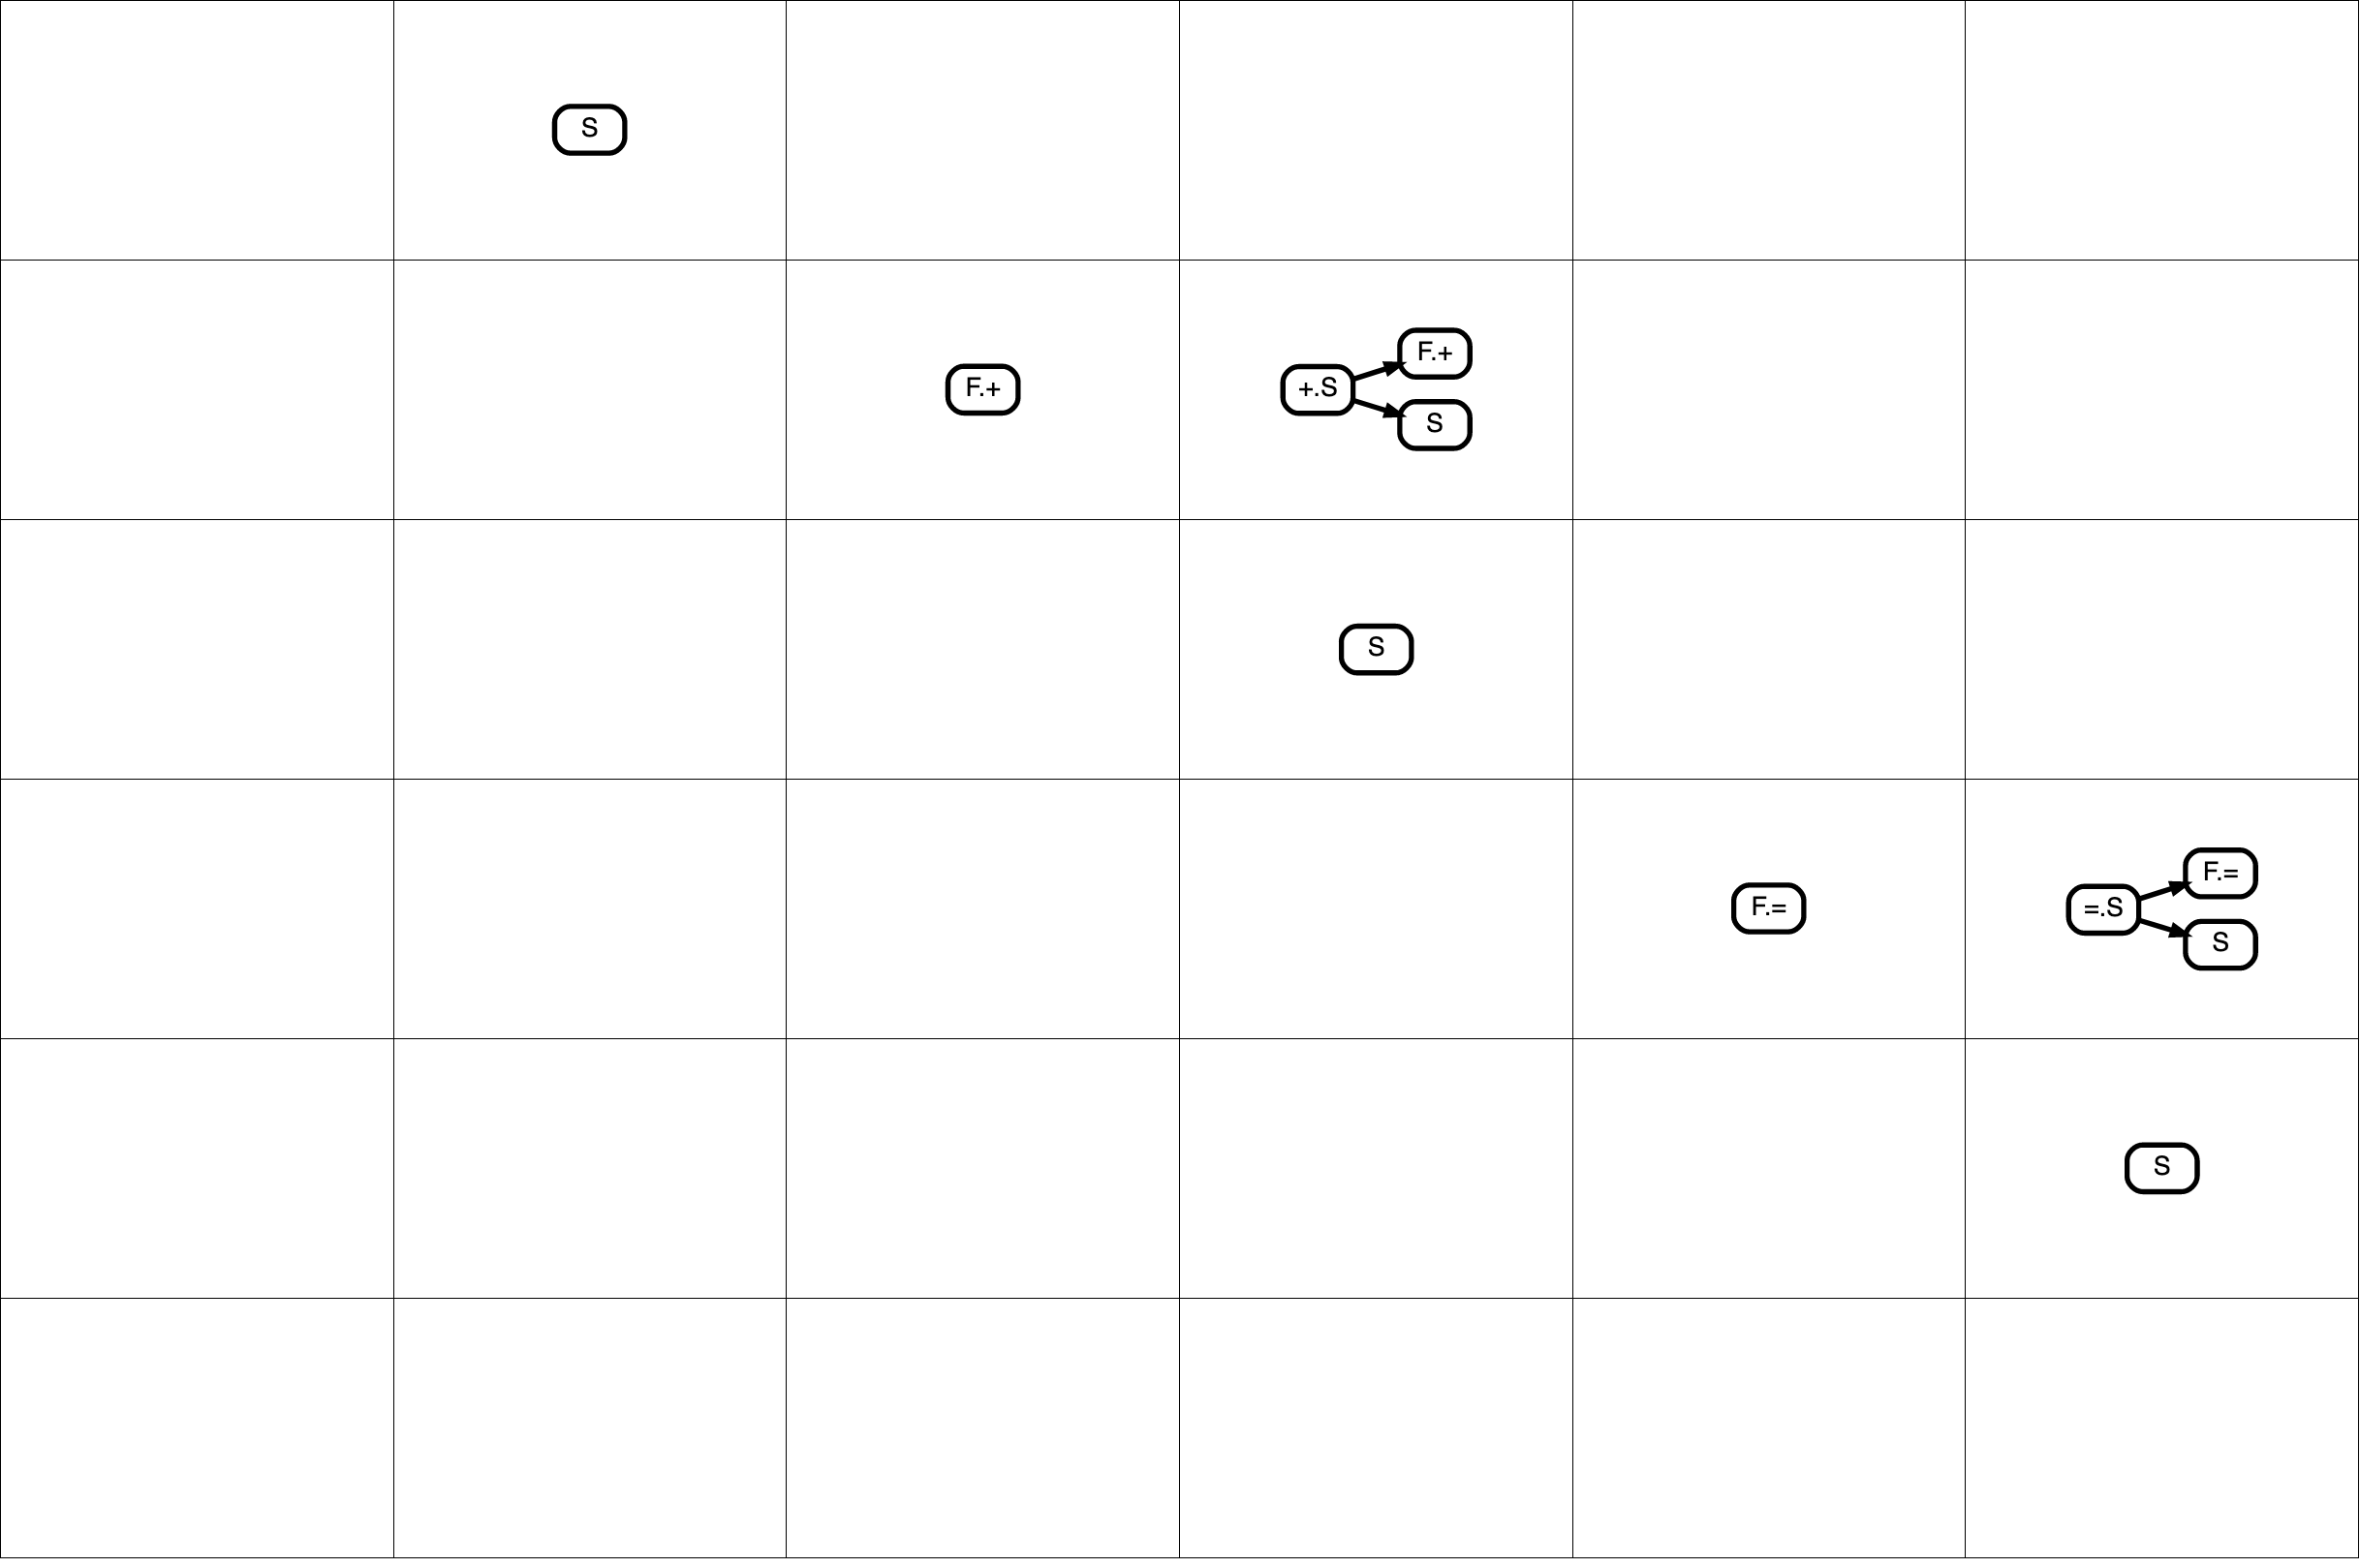
\includegraphics[trim=420 288 0 0,clip, width=12.24cm]{../figures/parse2.png} &
        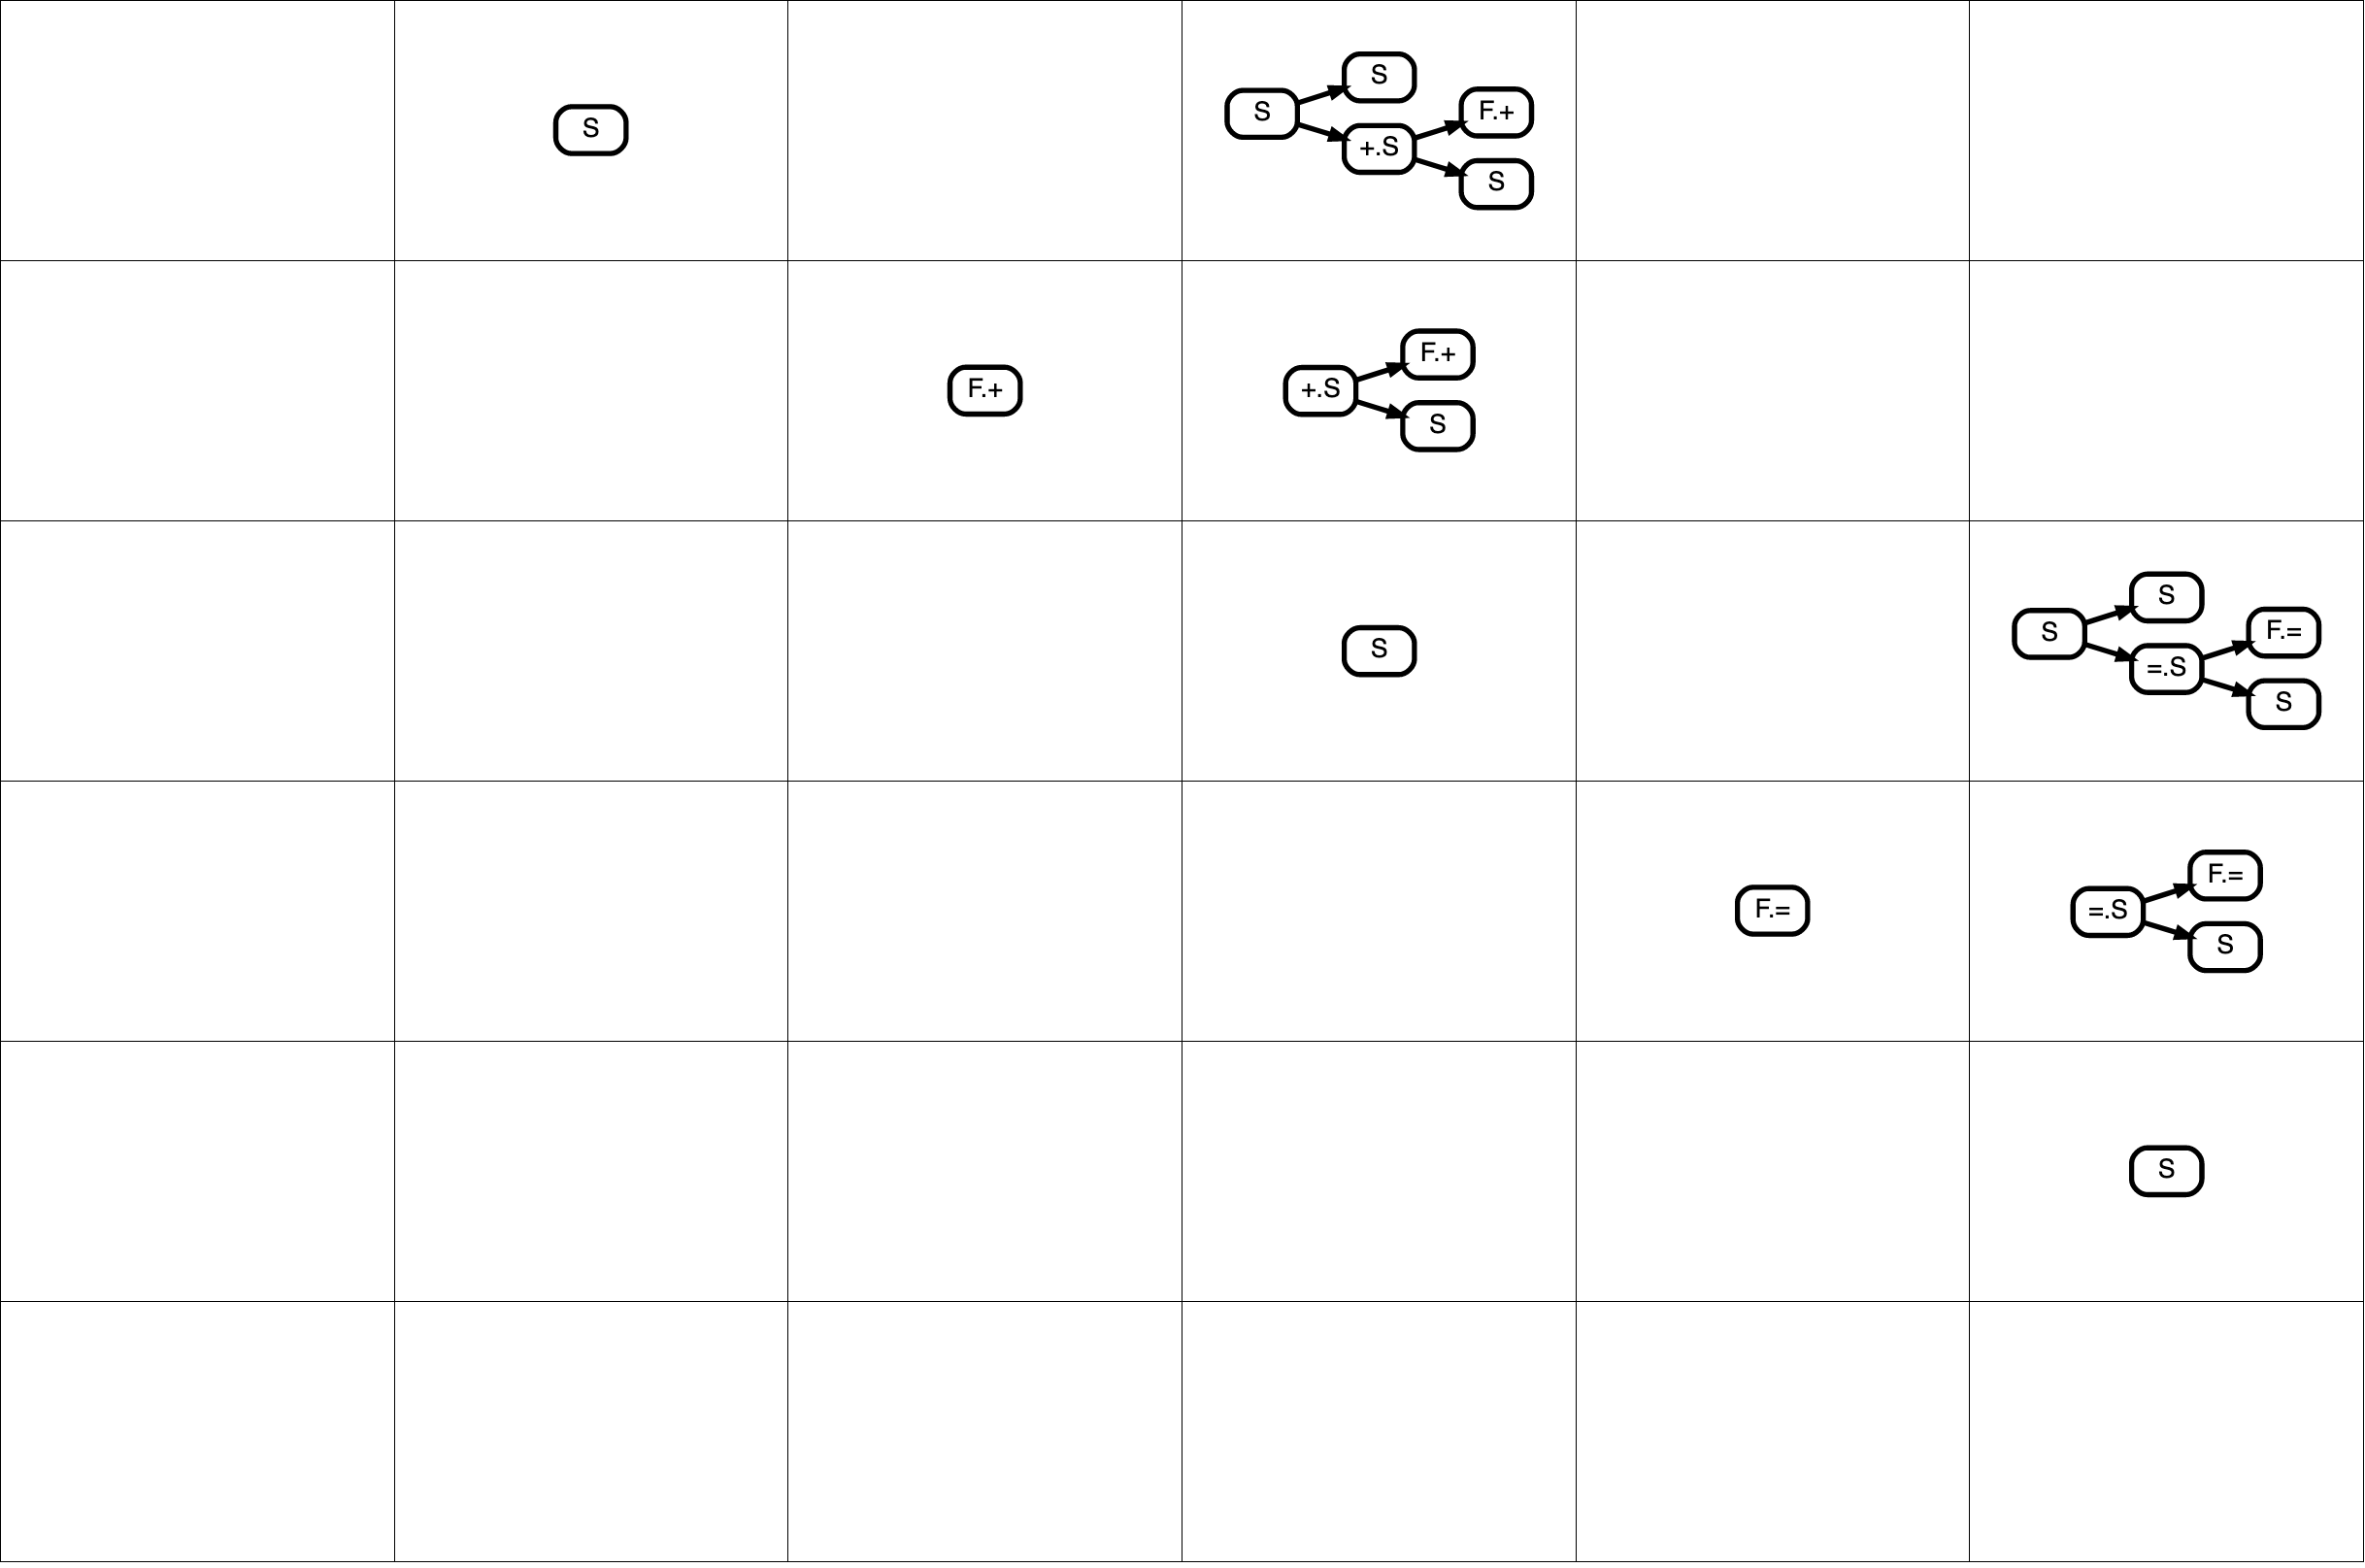
\includegraphics[trim=420 285 0 0,clip, width=12.24cm]{../figures/parse3.png} &
        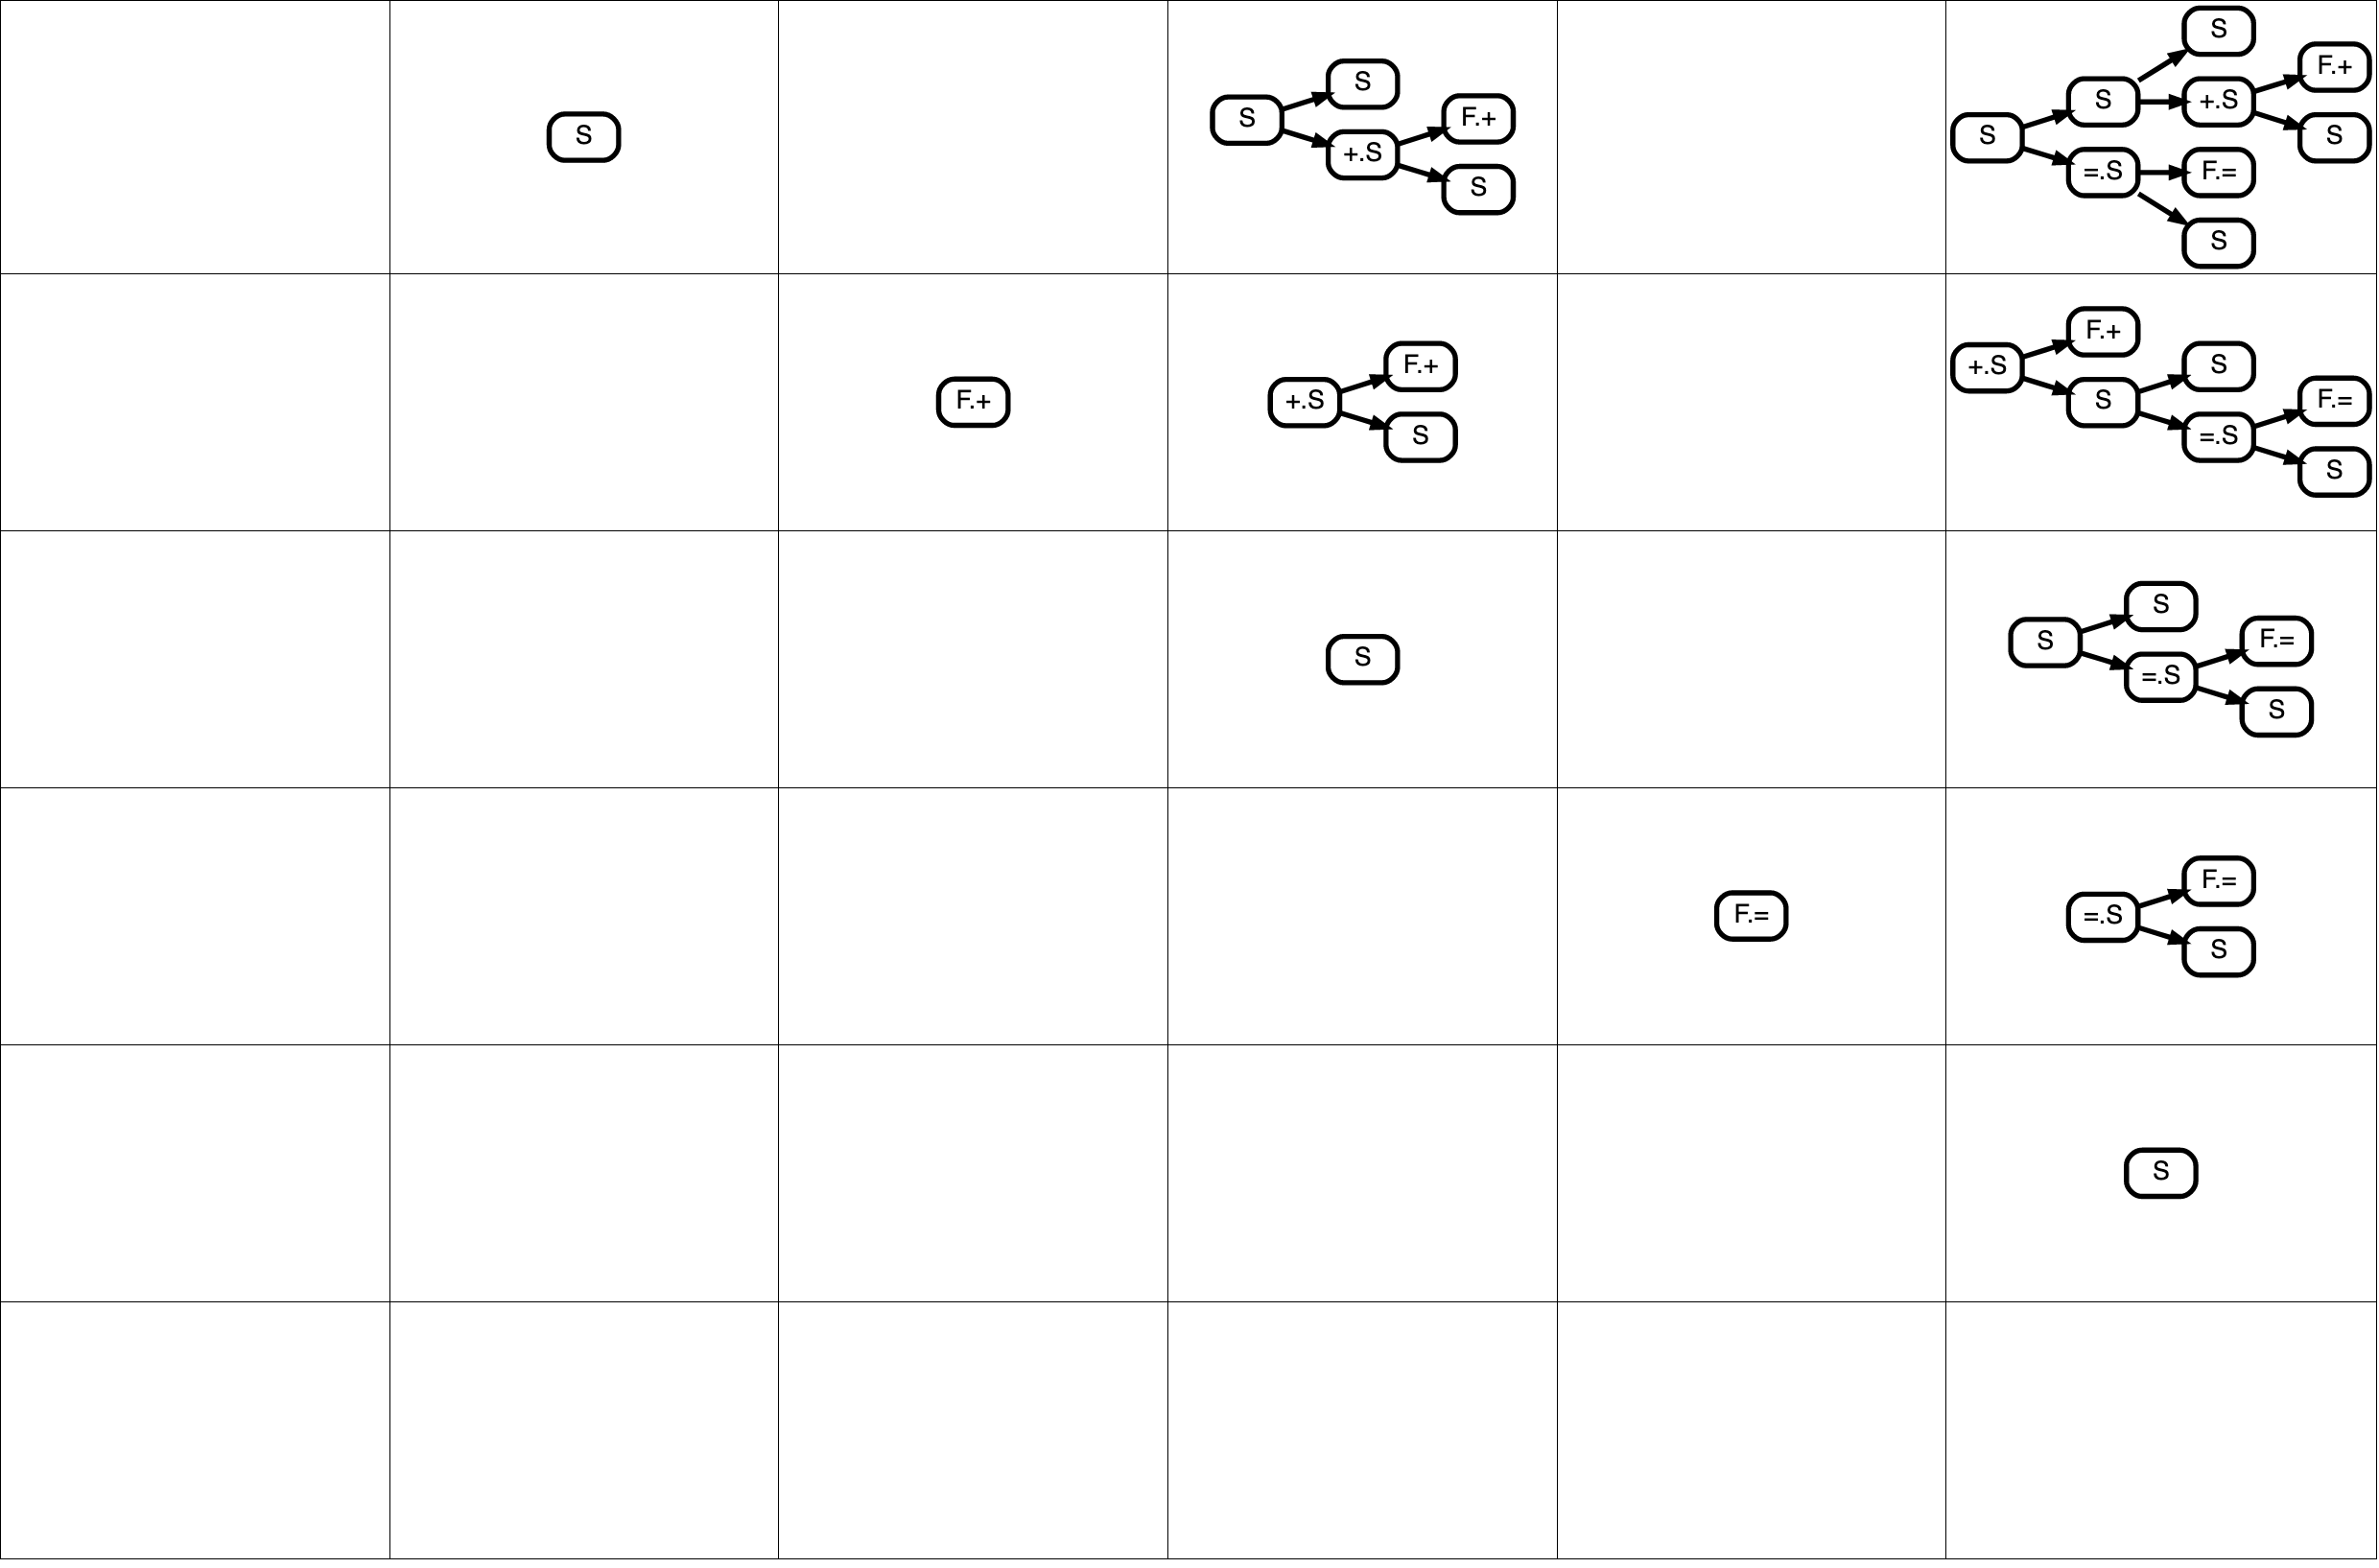
\includegraphics[trim=420 287 0 0,clip, width=12.34cm]{../figures/parse4.png}
      \end{tabular}
      \begin{itemize}
        \item If we had a way to solve for $\mathbf{M = M + M}^2$ directly, power iteration would be unnecessary and we could solve for $\mathbf{M = M}^2$ above the superdiagonal\ldots
      \end{itemize}
      \end{minipage}
      \jointspacing

      \mysection{Binarized CFL Sketching}
      \null\hspace*{3cm}\begin{minipage}[c]{0.90\columnwidth}
      \begin{itemize}
        \item CYK parser can be lowered onto a Boolean tensor $\mathbb{B}^{n\times n \times |V|}$ (Valiant, 1975)
        \item Binarized CYK parser can be compiled to SAT to solve for $\mathbf{M}^*$ directly
        \item Enables sketch-based synthesis in either $\sigma$ or $\mathcal G$: just use variables for holes!
        \item We simply encode the characteristic function, i.e. $\mathds{1}_{\subseteq V}: V\rightarrow \mathbb{B}^{|V|}$
        \item $\oplus, \otimes$ are defined as $\boxplus, \boxtimes$, so that the following diagram commutes:
        \[\begin{tikzcd}
            2^V \times 2^V \arrow[r, "\oplus/\otimes"] \arrow[d, "\mathds{1}^2"]
            & 2^V \arrow[d, "\mathds{1}\phantom{^{-1}}"] \\
            \mathbb{B}^{|V|} \times \mathbb{B}^{|V|} \arrow[r, "\boxplus/\boxtimes", labels=below] \arrow[u, "\mathds{1}^{-2}"]
            & \mathbb{B}^{|V|} \arrow[u, "\mathds{1}^{-1}"]
        \end{tikzcd}\]
        \item These operators can be lifted into matrices and tensors in the usual way
        \item In most cases, only a few nonterminals will be active at any given time
        \item More sophisticated representations are known for $\binom{n}{0 \leq k}$ subsets
%        \item If density is desired, possible to use the Maculay representation
%        \item If you know of a more efficient encoding, please let us know!
      \end{itemize}
      \end{minipage}

      \jointspacing

      \mysection{Feedback Shift Registers}

      \hspace*{2cm}\begin{minipage}[c]{0.90\columnwidth}
      Let $\textbf{M}: \text{GF}(2^{n\times n})$ be a square matrix $\mathbf{M}^0_{r, c} = P_c \text{ if } r=0 \text{ else } \mathds{1}[c = r - 1]$, where $P$ is a feedback polynomial with coefficients $P_{1\ldots n}$ and $\oplus := \veebar, \otimes := \land$:\\
      \end{minipage}

      \[
        \mathbf{M}^tV = \begin{pmatrix}
                          P_1 & P_2 & P_3 & P_4 & P_5 \\
                          \top & \circ & \circ & \circ & \circ \\
                          \circ & \top & \circ & \circ & \circ \\
                          \circ & \circ & \top & \circ & \circ \\
                          \circ & \circ & \circ & \top & \circ
        \end{pmatrix}^t
        \begin{pmatrix}
          V_1 \\
          V_2 \\
          V_3 \\
          V_4 \\
          V_5
        \end{pmatrix}
      \]\\

      \hspace*{2cm}\begin{minipage}[c]{0.90\columnwidth}
      Selecting any $V \neq \mathbf{0}$ and coefficients $P_j$ from a known \textit{primitive polynomial}, then powering the matrix $\mathbf{M}$ generates an ergodic sequence over GF$(2^n)$:
      \end{minipage}

      \[
        \mathbf{S} = \begin{pmatrix}V & \mathbf{M}V & \mathbf{M}^{2}V & \mathbf{M}^{3}V & \cdots & \mathbf{M}^{2^n-1}V \end{pmatrix}
      \]

      \hspace*{2cm}\begin{minipage}[c]{0.90\columnwidth}
      This sequence has \textit{full periodicity}, i.e., for all $i, j \in [0, 2^n), \mathbf{S}_i = \mathbf{S}_j \Rightarrow i = j$.
      \end{minipage}

      \jointspacing

      \mysection{Typelevel Modular Arithmetic}

      \hspace*{3cm}\begin{minipage}[c]{0.90\columnwidth}
      \begin{prooftree}
        \AxiomC{
          \phantom{\begin{tikzpicture}
                     \tige{1}{0}{0}
                     \barres{1}
          \end{tikzpicture}$_n+10^n$}
        }
        \UnaryInfC{
          \begin{tikzpicture}
            \tige{1}{0}{0}
            \tige{2}{0}{0}
            \tige{3}{0}{0}
            \cadre{3}
          \end{tikzpicture}
        }
        \DisplayProof
        \hskip 1em
        \AxiomC{
          \begin{tikzpicture}
            \tige{1}{0}{0}
            \barres{1}
          \end{tikzpicture}$_n+10^n$
        }
        \UnaryInfC{
          \begin{tikzpicture}
            \tige{1}{1}{0}
            \barres{1}
          \end{tikzpicture}$_n\phantom{n+0^n}$
        }
        \DisplayProof
        \hskip 1em
        \AxiomC{
          \begin{tikzpicture}
            \tige{1}{4}{0}
            \barres{1}
          \end{tikzpicture}$_n+10^n$
        }
        \UnaryInfC{
          \begin{tikzpicture}
            \tige{1}{5}{0}
            \barres{1}
          \end{tikzpicture}$_n\phantom{n+0^n}$
        }
        \DisplayProof
        \hskip 1em
        \AxiomC{
          \begin{tikzpicture}
            \tige{1}{0}{0}
            \barres{1}
            \tige[2]{1}{9}{0}
            \barres[2]{1}
          \end{tikzpicture}$_n+10^n$
        }
        \UnaryInfC{
          \begin{tikzpicture}
            \tige{1}{1}{0}
            \barres{1}
            \tige[2]{1}{0}{0}
            \barres[2]{1}
          \end{tikzpicture}$_n\phantom{n+0^n}$
        }
      \end{prooftree}
      \end{minipage}

%      \null\hspace*{3cm}\begin{minipage}[c]{0.85\columnwidth}Kotlin$\nabla$ is capable of computing arbitrarily high order derivatives.\end{minipage}\\
      \null\hspace*{2.1cm}\begin{minipage}[c]{0.90\columnwidth}
\begin{kotlinlisting}
// Typelevel Church encoding of dependently typed binary arithmetic
val t: T<T<T<T<F<T<O>>>>>> = T.F.T * T.F.F.T + T.F.T - T.T.F / T.F

// Typelevel Fibonacci configuration linear feedback shift register
val lfsr5 = BVec(T, F, F, T, T)
   .lfsr().lfsr().lfsr().lfsr().lfsr().lfsr() // BVec5<_, _, T, T, T>
   .lfsr().lfsr().lfsr().lfsr().lfsr().lfsr() // BVec5<T, T, _, T, T>
   .lfsr().lfsr().lfsr().lfsr().lfsr().lfsr() // BVec5<_, T, _, T, _>

// Typelevel implementation of Rule 110 elementary cellular automaton
val eca10 = BVec(T, T, F, F, F, T, F, F, F, F)
   .eca(::r110, ::r110, ...)  // BVec10<T, T, _, _, T, T, _, _, _, T>
   .eca(::r110, ::r110, ...)  // BVec10<T, T, _, T, T, T, _, _, T, T>
   .eca(::r110, ::r110, ...)  // BVec10<T, T, T, T, _, T, _, T, T, T>
   .eca(::r110, ::r110, ...)  // BVec10<_, _, _, T, T, T, T, T, _, _>
\end{kotlinlisting}
      \end{minipage}

      \jointspacing

      \mysection{Tidyparse IDE Plugin}

      \null\hspace*{1.8cm}\begin{minipage}[c]{0.90\columnwidth}
          \href{https://github.com/breandan/tidyparse}{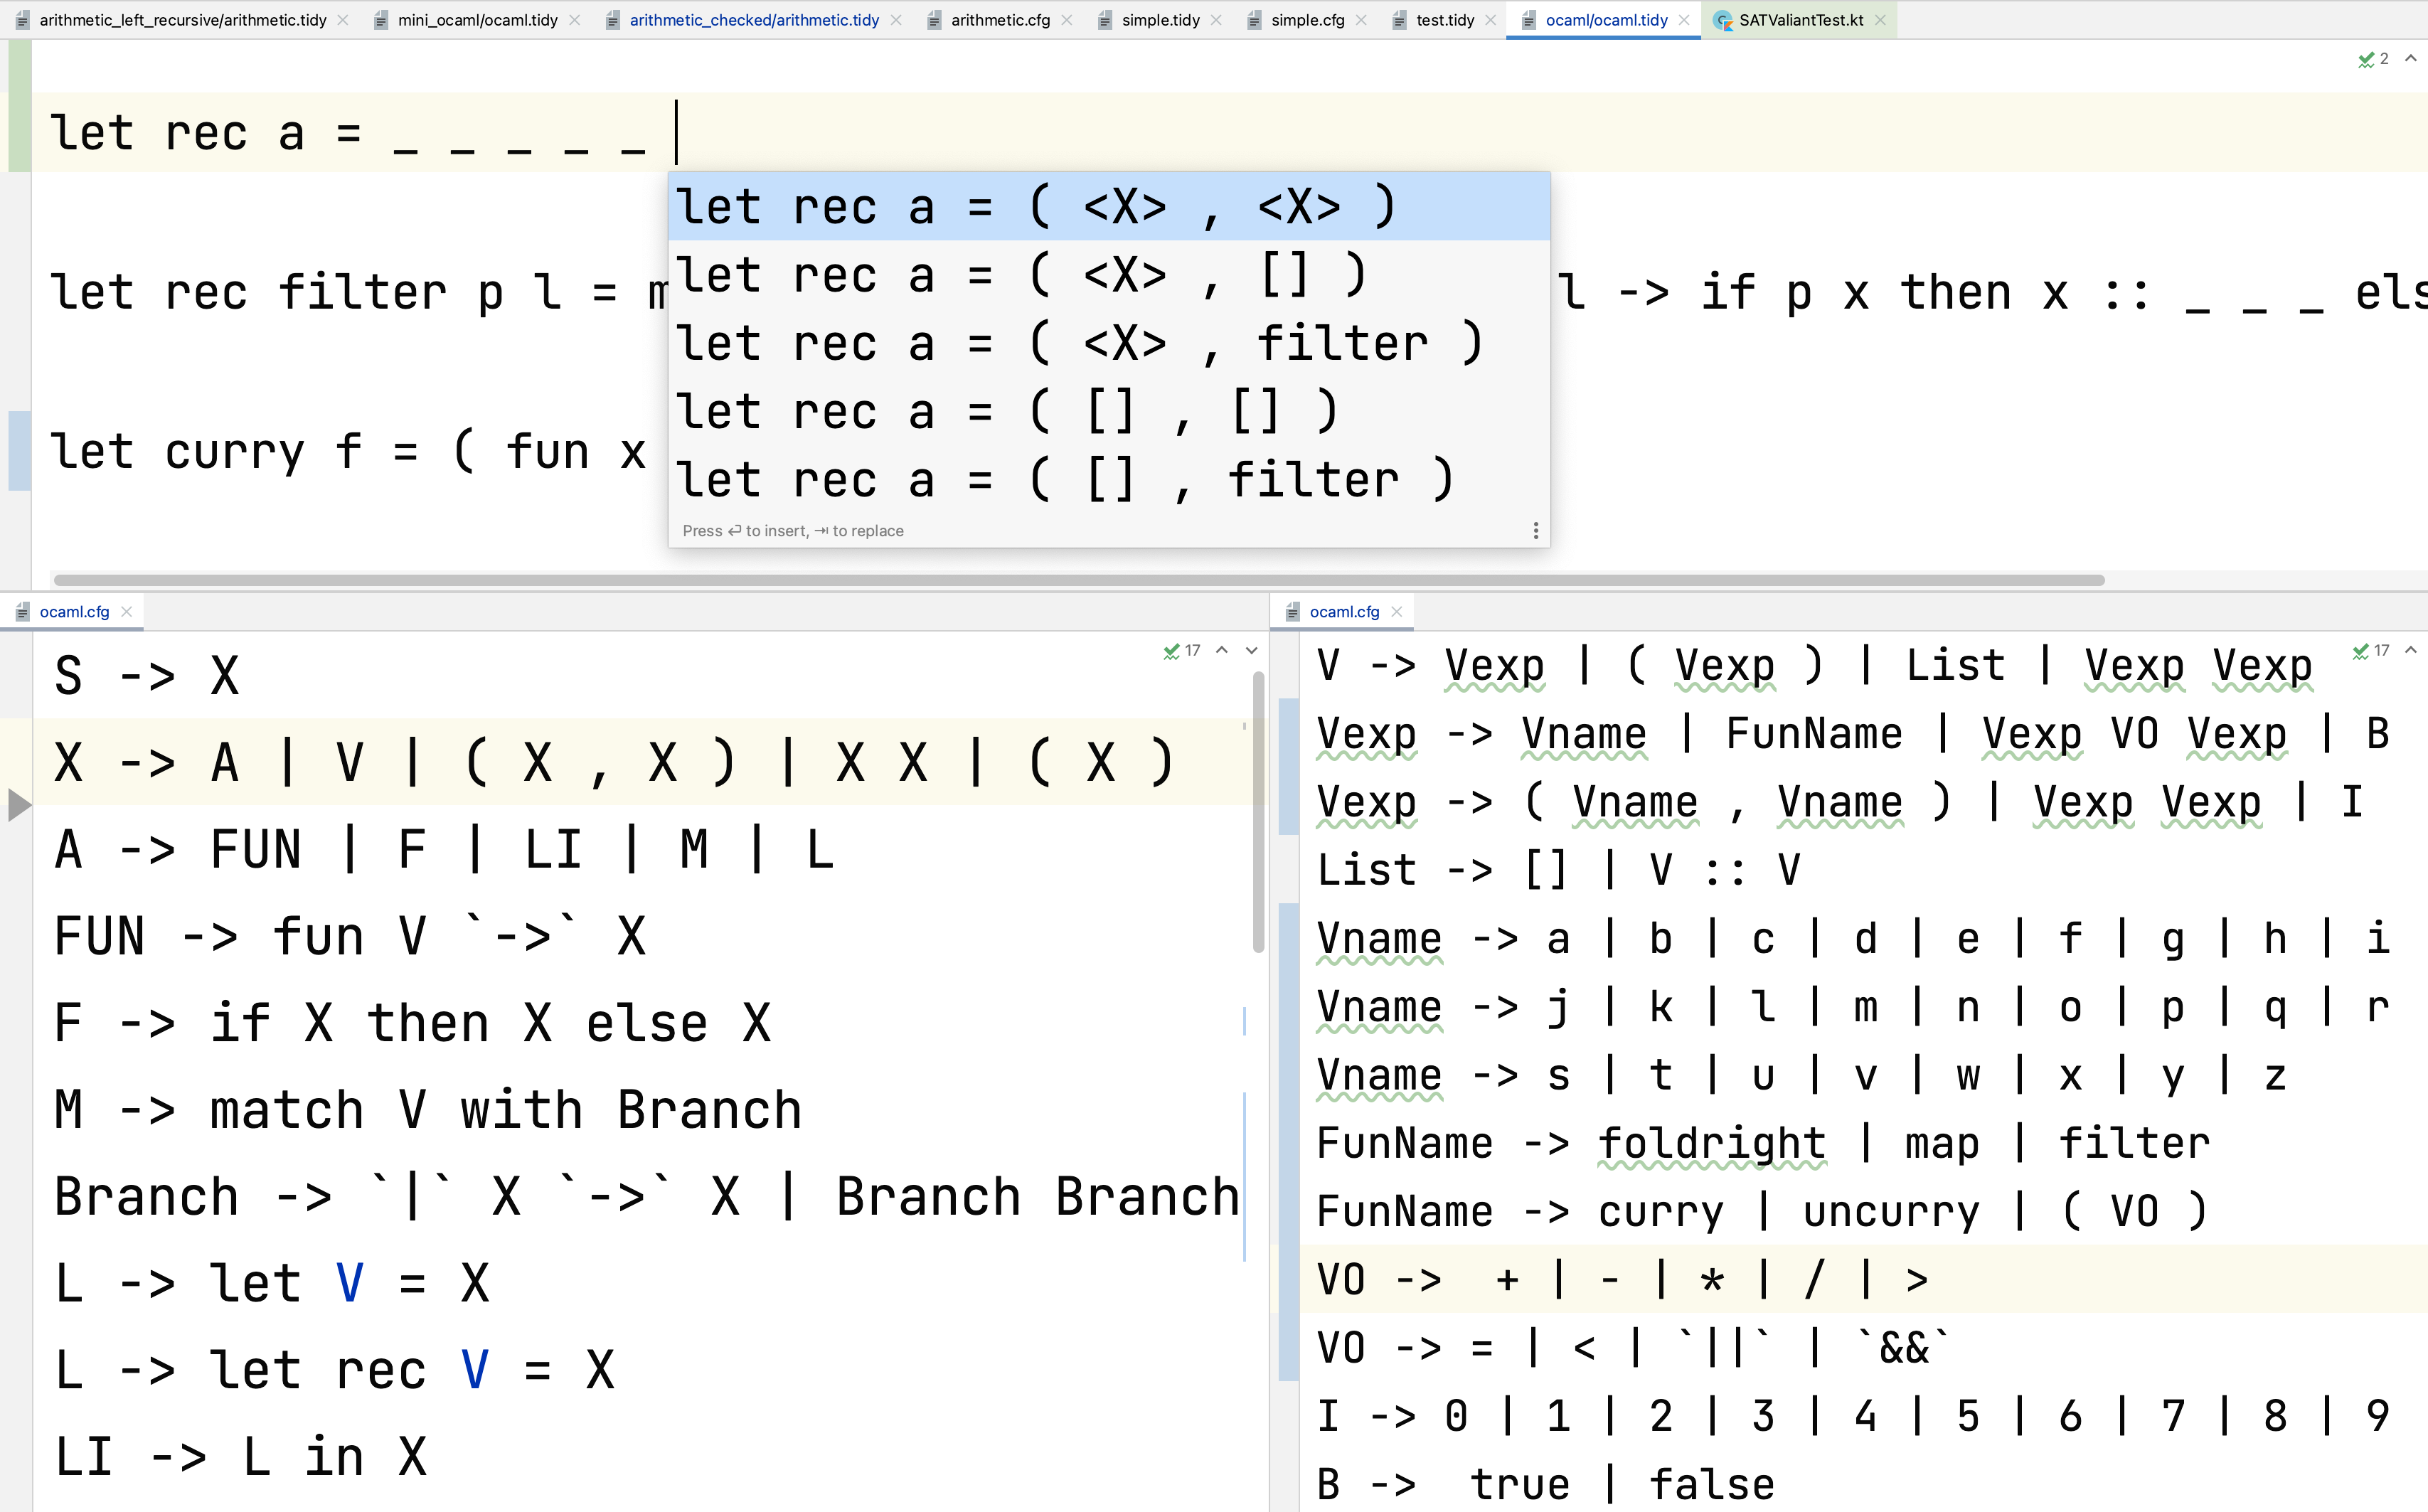
\includegraphics[width=\textwidth]{../figures/tidyparse.png}}
      \end{minipage}

      \jointspacing

    \end{multicols}

    \bottombox{
    %% QR code
    %    \hfill\bottomboxlogo{img/kotlin_logo.png}
    % Comment out the line below out to hide logo
    \begin{minipage}[c][0.1\paperheight][c]{0.18\textwidth}\qrcode[height=2.6in]{ssnp.ndan.co} \end{minipage}
    \begin{minipage}[c][0.1\paperheight][c]{0.25\textwidth}
\includegraphics[height=2.6in]{../figures/fpt_logo.png} \end{minipage}
    \begin{minipage}[c][0.1\paperheight][c]{0.33\textwidth}
\includegraphics[height=2.6in]{../figures/mcgill.png} \end{minipage}
    \begin{minipage}[c][0.1\paperheight][c]{0.33\textwidth}
\includegraphics[height=3.2in]{../figures/mila.png} \end{minipage}
    %    \hfill\bottomboxlogo{img/mila_mauve.png} % \hfill shifts the logo across so it meets the right hand side margin
    % Note that \bottomboxlogo takes an optional width argument. It defaults to the following:
    % \hfill\bottomboxlogo[width=\textwidth]{<path_to_image_file>}
    % where \textwidth is actually the width of a minipage which is defined in the \bottombox command of
    % betterportaitposter.cls It's a standard \includegraphics command in there, so easy to change if
    % you need to add a border etc.
    }
\end{poster}
\end{document}
